\documentclass[11pt,letterpaper]{article}
\usepackage[utf8]{inputenc}
\usepackage{amsmath}
\usepackage{amsfonts}
\usepackage{amssymb}
\usepackage{geometry}
\usepackage{hyperref}
\usepackage{xcolor}
\usepackage{booktabs}
\usepackage{multicol}
\usepackage{caption}
\usepackage{float}
\usepackage{graphicx}
\graphicspath{{visual-assets/}}

% Brand Typography / Color configuration
\definecolor{mpdark}{HTML}{0F172A}
\definecolor{mpblue}{HTML}{3B82F6}
\definecolor{mpgreen}{HTML}{10B981}
\definecolor{mpred}{HTML}{EF4444}
\definecolor{mppurple}{HTML}{8B5CF6}
\definecolor{mpamber}{HTML}{F59E0B}
\definecolor{mpgrey}{HTML}{64748B}

\geometry{margin=1in}

\hypersetup{
    colorlinks=true,
    linkcolor=mpblue,
    urlcolor=mpblue
}

\setlength{\abovedisplayskip}{4pt}
\setlength{\belowdisplayskip}{4pt}
\setlength{\abovedisplayshortskip}{2pt}
\setlength{\belowdisplayshortskip}{2pt}

\newcommand{\plain}[1]{\par\smallskip\noindent\textcolor{mpgrey}{\textit{In plain terms:} #1}\par\smallskip}

\title{\vspace{-20pt}\textbf{\color{mpdark}Money Plot Labs Technical Whitepaper 005 \\
Spending Strategies and Quality of Life: \\
How the Strategy Lab Scores and Optimizes Retirement Spending}}
\author{\textbf{Money Plot Labs}}
\date{October 2026}

\begin{document}

\maketitle

\begin{abstract}
\vspace{-5pt}
The Stress Tester (Whitepaper 003) asks whether a \emph{fixed} spending plan survives market volatility. The Spending Strategy Lab asks a different question: \emph{given the same markets, which way of setting retirement spending buys the best life?} This paper documents every calculation behind the Lab so that none of it is a black box. We specify the year-by-year simulation kernel (including the rule that balances never go below \$0), the five spending strategies --- Fixed, Constant~\%, Amortization (VPW), Guardrails and Optimal --- and the quality-of-life score that ranks them: a happiness curve anchored at the spending you planned, weighted by survival odds, and converted back into a ``steady-spend equivalent'' in dollars. Finally we derive the Optimal strategy as the solution of a dynamic program that maximizes that score, describe its numerical method and validation, and work through a complete example.
\end{abstract}

% =========================================================================
\section{What the Strategy Lab Computes}
% =========================================================================

For one set of inputs (milestones, Social Security, windfalls, recurring expenses, retirement trigger, growth methods) the Lab:
\begin{enumerate}
\setlength\itemsep{1pt}
\item draws one set of return sequences --- 1{,}000 bootstrap runs, or the chronological cohorts (Whitepaper 003);
\item runs \emph{every} strategy on \emph{those same sequences}, so differences between strategies come only from the spending rule;
\item scores every run with the quality-of-life model of Section~\ref{sec:qol} and summarizes each strategy (Section~\ref{sec:metrics});
\item charts the selected strategy: the net-worth percentile fan, the representative downside run, and that run's cash flows.
\end{enumerate}
All amounts are in real (today's) dollars and returns are real, as in the rest of the suite.

% =========================================================================
\section{The Simulation Kernel}
\label{sec:kernel}
% =========================================================================

\subsection{Notation}

Ages run from the current age $t_0$ to the planning horizon $T$ (the ``Life Expectancy'' input). For each age $t$:

\begin{center}
\begin{tabular}{@{}ll@{}}
\toprule
$B_t$ & portfolio at the start of year $t$ ($B_{t_0}$ = starting balance) \\
$a_t,\; r_t$ & real return in year $t$ while working / once retired (the two growth methods) \\
$s_t$ & milestone savings minus working-years recurring expenses \\
$w_t$ & milestone lifestyle spending plus working-years recurring expenses \\
$\bar c_t$ & milestone lifestyle spending plus retired-years recurring expenses (the plan once retired) \\
$P_t$ & Social Security / pensions that have started by age $t$ \\
$W_t$ & one-time windfall at age $t$ (zero in other years) \\
$R$ & retirement age; $k=\lfloor R\rfloor$, $\delta = R-k$ \\
\bottomrule
\end{tabular}
\end{center}

The fraction of year $t$ worked is
\begin{equation}
\omega_t = \begin{cases} 1 & t < k \\ \delta & t = k \\ 0 & t > k \end{cases}
\end{equation}
so the retirement year is split between a worked part ($\omega_t$) and a retired part ($1-\omega_t$).

\paragraph{Retirement age.} With ``Retire at Age'', $R$ is the input. With ``Retire at Net Worth'' (target $N^\star$), $R$ is the first crossing during accumulation: if $B_t < N^\star \le B_t(1+a_t)+s_t+P_t+W_t$ then $R = t + (N^\star - B_t)/\big(B_t(1+a_t)+s_t+P_t+W_t - B_t\big)$, clamped to $[t, t+1]$. Strategies never change $R$: every strategy retires at the same age in the same run.

\subsection{One Year}

\textbf{Worked part.} Pay covers lifestyle spending; savings, pensions and windfalls land at the end of the worked part:
\begin{equation}
M_t = B_t(1+a_t)^{\omega_t} + (s_t + P_t + W_t)\,\omega_t, \qquad \text{spent}_t = w_t\,\omega_t .
\end{equation}
If $M_t<0$ (negative savings with an empty portfolio), spending is cut by the shortfall and $M_t$ is set to 0.

\textbf{Retired part.} The strategy proposes an annual spending rate $d_t$ (Section~\ref{sec:strategies}), evaluated with balance $M_t$. Withdrawals happen at the start of the retired part, and can never exceed what is there:
\begin{align}
A_t &= M_t + (P_t + W_t)(1-\omega_t) && \text{(available)}\\
D_t &= \min\!\big(d_t(1-\omega_t),\; \max(0, A_t)\big) && \text{(withdrawn)}\\
I_t &= \max(0,\, A_t - D_t) && \text{(left invested)}\\
B_{t+1} &= I_t\,(1+r_t)^{1-\omega_t}
\end{align}
and $\text{spent}_t \mathrel{+}= D_t + \min(0, A_t)$ (an unpayable negative windfall also cuts spending).

\textbf{Growth} (the purple bars) is the investment return earned that year:
\begin{equation}
G_t = B_t\big[(1+a_t)^{\omega_t}-1\big] + I_t\big[(1+r_t)^{1-\omega_t}-1\big].
\end{equation}

\plain{balances stop at \$0 instead of going into debt, and an empty portfolio earns nothing. Once the money is gone, a run can only spend that year's Social Security, windfalls or pay.}

\subsection{Running Out and Success}

A run \emph{runs out} at the first age where it spent less than the strategy asked for (by more than \$1):
\begin{equation}
\text{ranOutAge} = \min\{\,t : \text{spent}_t < w_t\omega_t + d_t(1-\omega_t) - 1\,\}.
\end{equation}
A run is a \textbf{success} if it never runs out \emph{and} ends at or above the Desired Legacy Floor (with a \$1 tolerance). The flexible strategies below never ask for more than is available, so they never run out; their success depends only on the legacy floor.

The plan's spending for the ``below plan'' statistics is $\text{planned}_t = w_t\omega_t + \bar c_t(1-\omega_t)$.

% =========================================================================
\section{The Five Spending Strategies}
\label{sec:strategies}
% =========================================================================

Each strategy returns $d_t$, the year's \emph{total} spending (portfolio withdrawals plus pensions), given the balance $B=M_t$ at the start of the retired part. Before retirement every strategy spends the milestone plan; they differ only in retirement.

\subsection{Fixed}
\begin{equation}
d_t = \bar c_t .
\end{equation}
Spend the plan regardless of markets. This is the Stress Tester's model; it is the only strategy that can run out.

\subsection{Constant Percentage}
\begin{equation}
d_t = q\,\max(0,B) + P_t, \qquad q = \text{Withdrawal Rate (default 4\%)}.
\end{equation}
Never runs out, but spending moves one-for-one with the portfolio. Windfalls are not spent directly; they join the portfolio.

\subsection{Amortization (VPW)}
Each year, re-solve for the level spending that would use up the portfolio \emph{plus} the present value of all future pensions and windfalls by the horizon, if the portfolio earned the Assumed Real Return $g$ (default 4\%):
\begin{equation}
\mathrm{PV}_t = \sum_{j=t}^{T} \frac{P_j + W_j}{(1+g)^{\,j-t}}, \qquad
d_t = \mathcal{A}\!\big(\max(0,B) + \mathrm{PV}_t,\; g,\; T-t+1\big),
\end{equation}
where $\mathcal{A}$ is the payment at the \emph{start} of each of $n$ years that exhausts $X$:
\begin{equation}
\mathcal{A}(X, g, n) = \frac{X\,g}{\big(1-(1+g)^{-n}\big)(1+g)}, \qquad \mathcal{A}(X,0,n) = X/n .
\end{equation}
If returns match $g$ exactly, spending is level for life and the balance reaches \$0 at the horizon. Counting future Social Security as wealth smooths spending across its start date --- but because the portfolio cannot borrow against it, a bad early sequence can still leave a lean stretch before Social Security begins (see the cap below).

\subsection{Guardrails (simplified Guyton--Klinger)}
Spending is the plan times a multiplier $m$ (starting at 1). In the first retired year the initial withdrawal rate is recorded:
\begin{equation}
\mathrm{WR}_0 = \frac{\bar c_t - P_t}{B} \qquad (0 \text{ if } B \le 0).
\end{equation}
In each later year, before spending, the current rate $\mathrm{wr} = (m\,\bar c_t - P_t)/B$ is compared with the band $b$ (default 20\%) and the multiplier adjusted by $\alpha$ (default 10\%):
\begin{equation}
m \leftarrow \begin{cases} m(1-\alpha) & \mathrm{wr} > \mathrm{WR}_0(1+b) \\ m(1+\alpha) & \mathrm{wr} < \mathrm{WR}_0(1-b) \\ m & \text{otherwise} \end{cases}
\qquad d_t = m\,\bar c_t .
\end{equation}
This is a real-terms simplification: there is no separate inflation-skip rule and no capital-preservation sunset. Because $\mathrm{WR}_0$ is measured at retirement, a pension that starts years later lowers the withdrawal rate and can trigger a run of raises.

\subsection{Optimal}
\begin{equation}
d_t = \pi_t\big(\max(0,B) + P_t + W_t\big),
\end{equation}
where $\pi_t(X)$ is the spending policy that maximizes the quality-of-life score, derived in Section~\ref{sec:dp}.

\subsection{The No-Borrowing Cap}
Every flexible strategy (all but Fixed) is capped so it never asks for more than the year can fund:
\begin{equation}
d_t \leftarrow \max\!\Big(0,\; \min\!\big(d_t,\; \max(0,B)/(1-\omega_t) + P_t + W_t\big)\Big).
\end{equation}

% =========================================================================
\section{The Quality-of-Life Score}
\label{sec:qol}
% =========================================================================

Success rate treats a run that trims spending by 1\% the same as one that never trims, and a run that runs out at 94 the same as one that runs out at 60. The quality-of-life score instead values \emph{the spending each run actually delivered}, year by year.

\subsection{The Target Happiness Curve (default)}
Each year has a \textbf{target} $\tau_t$: the plan's spending that year --- milestone lifestyle spending plus the recurring expenses that apply (working-years rows in working years, retired-years rows once retired). With spending $c_t$, define the share of plan $x = c_t/\tau_t$, the floor share $f = \min(F/\tau_t,\,0.9)$ for the Spending Floor $F$, and $\kappa = \lambda(1-f)$ for the Shortfall Pain $\lambda \ge 1$. Happiness is
\begin{equation}
u(c_t) = \begin{cases}
\dfrac{x^{1-\eta}-1}{1-\eta} \quad (\ln x \text{ if } \eta=1) & x \ge 1 \quad\text{(above plan)}\\[8pt]
\kappa\,\ln\!\dfrac{x-f}{1-f} & x_m \le x < 1 \quad\text{(below plan)}\\[8pt]
\kappa\ln\!\dfrac{x_m-f}{1-f} + \dfrac{\kappa}{x_m-f}\,(x-x_m) & x < x_m \quad\text{(near/below the floor)}
\end{cases}
\end{equation}
with $x_m = \min\!\big(f + \$1{,}000/\tau_t,\; (1+f)/2\big)$. Its properties:
\begin{itemize}
\setlength\itemsep{1pt}
\item $u = 0$ exactly at the plan, so a run that always spends the plan scores 100\%.
\item Per dollar, the slope just below the plan is $\lambda$ times the slope just above it: at $\lambda = 2.5$, a small cut of \$1{,}000 hurts like a \$2{,}500 raise helps. Deeper cuts hurt faster, steeply as spending approaches the floor; within \$1{,}000 of the floor the penalty continues as a steep straight line, so one bad year is very costly but cannot outweigh everything else.
\item Above the plan, gains diminish at a rate set by Extra Spending Worth: High ($\eta = 1$, each doubling adds the same), Moderate ($\eta=2$, default; doubling the plan gives half of all the upside there is) or Low ($\eta=4$). For $\eta>1$ the upside is capped at $1/(\eta-1)$.
\item The curve is increasing and concave, which the optimizer needs.
\end{itemize}

\begin{figure}[H]
\centering
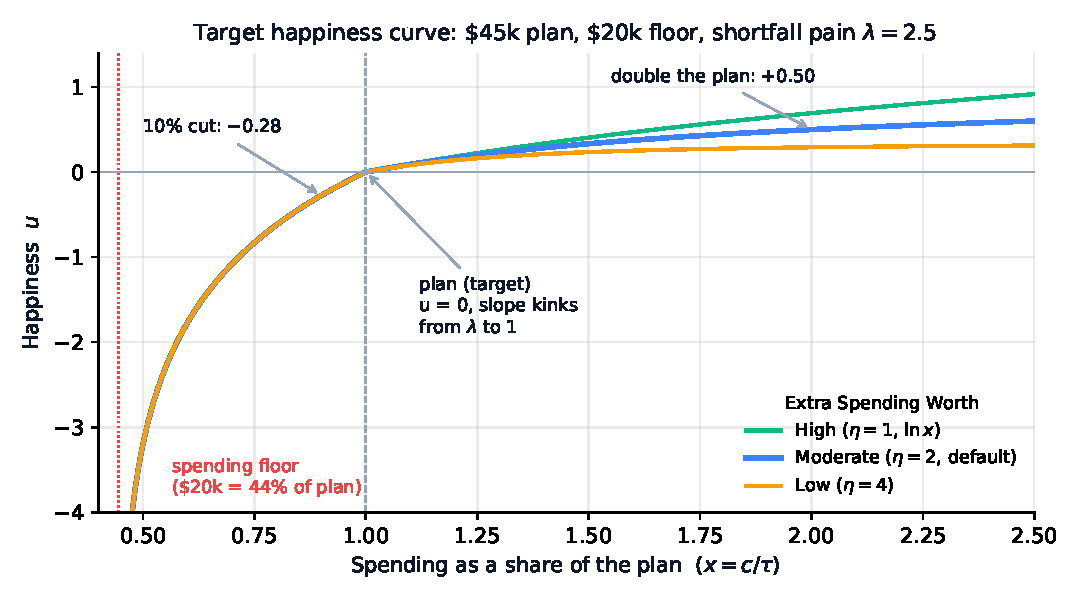
\includegraphics[width=0.86\linewidth]{target_utility.pdf}
\caption{The target happiness curve with the tool's defaults. A 10\% cut costs $0.28$; it takes a 38\% raise to earn that back, and doubling the plan for a year only makes up for a 17\% cut.}
\end{figure}

\paragraph{Calibration line.} Under the inputs, the Lab prints what the settings mean at the plan's spending at the current age: the raise $\rho$ that offsets a 10\% cut, and the cut $z$ that a year at double the plan offsets,
\begin{equation}
u\big((1+\rho)\tau\big) = -u(0.9\,\tau), \qquad u\big((1-z)\tau\big) = -u(2\tau),
\end{equation}
solved by bisection. With the defaults ($\lambda=2.5$, $\eta=2$, \$20k floor, \$45k plan): $\rho = 38\%$ and $z = 17\%$. If no raise can offset the cut (the cut exceeds the upside cap), it says so.

\subsection{The Smooth-Curve Alternative}
Choosing ``Smooth curve ($\gamma$)'' replaces the target with constant relative risk aversion above the floor,
\begin{equation}
u(c) = \frac{(c-F)^{1-\gamma}}{1-\gamma} \quad (\ln(c-F) \text{ if } \gamma = 1),
\end{equation}
again continued linearly below $F + \$1{,}000$. $\gamma$ is the Swing Aversion (default 2). This model has no target and no leftover-money value.

\subsection{Weighting the Years}
Year $t$ (counted from the current age) gets weight
\begin{equation}
\varpi_t = \beta^{\,t-t_0}\; S_t\; a(t),
\end{equation}
\begin{itemize}
\setlength\itemsep{1pt}
\item $S_t$ --- probability of being alive at the start of year $t$: $S_{t_0} = 1$, $S_{t+1} = S_t(1-q_t)$. The one-year death rates $q_t$ are the CDC/NCHS \href{https://www.cdc.gov/nchs/data/nvsr/nvsr74/nvsr74-06.pdf}{United States Life Tables, 2023} (NVSR vol.~74 no.~6; data files: \href{https://ftp.cdc.gov/pub/Health_Statistics/NCHS/Publications/NVSR/74-06/Table02.xlsx}{males, Table~2} and \href{https://ftp.cdc.gov/pub/Health_Statistics/NCHS/Publications/NVSR/74-06/Table03.xlsx}{females, Table~3}) for ages 0--99, male, female, or their average (Unisex). The tables end in an open ``100 and older'' bracket, so ages 100--118 extend a Gompertz hazard fitted to ages 90--99, and $q_{119} = 1$. Unisex life expectancy at 65 is 19.4 years. ``Off'' --- the default --- sets $S_t = 1$ through the horizon: every year up to the horizon counts as if you will surely live it, which protects late-life spending most (a shortfall at 90 counts as much as one at 60, apart from the age weight and discount).
\item $\beta = 1/(1+d)$ --- the \textbf{Time Discount} $d$ per year. By default (\emph{Match expected return}) $d$ is the mean annual return $\mu$ of the model the Optimal strategy is solved against (Section~\ref{sec:dp}; 5.9\% for 60/40 history), so $\beta(1+\mu)=1$. With steady returns this makes the optimal spending path level: by the Euler condition $u'(c_t) = \beta\,\mathbb{E}[(1+r)\,u'(c_{t+1})]$, spending rises over time when returns beat the discount and falls when the discount beats returns. \emph{Custom} sets $d$ directly.
\item $a(t)$ --- \textbf{Enjoyment by age}: 1 until the ``declines from'' age $A$ (default 70), then linear to the ``enjoyment at 90'' value $e_{90}$ (default 100\%, i.e.\ no decline), held after 90.
\end{itemize}
Years past the horizon are never scored; with mortality on, when $S_{T+1} > 5\%$ the score card warns ``\% outlive horizon''.

\subsection{Leftover Money}
With the target model, wealth left at death --- or at the horizon --- is worth something. Let $\theta$ be Leftover \$ Worth (default 25\%), $L = 100$ years and $G(y) = \big((1+y)^{1-\eta}-1\big)/(1-\eta)$ ($\ln(1+y)$ if $\eta = 1$). Leaving wealth $W$ at age $t$ is worth
\begin{equation}
\mathcal{B}(W, t) = \theta\, L\; G\!\left(\frac{W}{L\,\tau^{\mathrm{ret}}_t}\right),
\end{equation}
where $\tau^{\mathrm{ret}}_t$ is the retired-years target. The first dollars left are worth $\theta$ of a dollar of extra spending at the plan ($\mathcal{B}'(0) = \theta/\tau$), and the value tapers with the same curvature as spending above the plan, over a scale of $L$ years of planned spending (at $\eta=2$, a leftover dollar keeps at least half its value until about 40 years' worth is left). Without this term, any surplus would eventually be spent (it is otherwise worthless); with an untapered (linear) value, plans that leave huge estates in good markets would dominate the score.

\subsection{Lifetime Score and Certainty Equivalent}
For one run, with end-of-year wealth $B_{t+1}$ and the probability of dying in year $t$, $\ell_t = S_t - S_{t+1}$ (and $\ell_T = S_T$, all remaining wealth being left at the horizon):
\begin{equation}
V = \sum_{t=t_0}^{T} \varpi_t\, u(c_t) \;+\; \sum_{t=t_0}^{T} \beta^{\,t-t_0+1}\,\ell_t\, \mathcal{B}(B_{t+1}, t).
\end{equation}
$V$ is converted back to dollars as a \textbf{certainty equivalent}: the steady spending, every year, that would score the same. With the average target $\bar\tau = \sum \varpi_t \tau_t / \sum \varpi_t$ and $u_{\bar\tau}$ the target curve at $\bar\tau$,
\begin{equation}
\mathrm{CE} = u_{\bar\tau}^{-1}\!\left(\frac{V}{\sum_t \varpi_t}\right), \qquad \text{\% of plan} = \mathrm{CE}/\bar\tau .
\end{equation}
(For the smooth curve, $\mathrm{CE} = u^{-1}(V/\sum\varpi_t)$.) A strategy's headline score uses the \emph{average} of $V$ over all runs before inverting, so market risk lowers it: by concavity, an uncertain outcome is worth less than its average. CE can exceed 100\% of plan when good markets allow spending above the plan or leave money behind.

\subsection{Summary Statistics}
\label{sec:metrics}
\begin{itemize}
\setlength\itemsep{1pt}
\item \textbf{Quality of Life} --- the across-run CE above, with its gap to the best strategy.
\item \textbf{10--90\%} --- the 10th and 90th percentiles of the per-run CEs.
\item \textbf{Retired Spend p10 / p50} --- percentiles of spending pooled over every fully retired year ($\omega_t=0$) of every run (not survival-weighted).
\item \textbf{Yrs Below Plan} --- per run, the years spending falls short of the plan by any amount over \$1, $n = \sum_t S_t\,\mathbf{1}[c_t < \text{planned}_t - 1]$ (with mortality off, $S_t = 1$ and this is a plain count). The table shows the average of $n$ over runs and its 90th percentile (the worst 10\% of runs have at least that many); the score card also shows $n$ for the charted downside run. That run is chosen by quality of life, not by $n$, so it can have more below-plan years than the 90th percentile: many small trims can score better than a few deep cuts. For flexible strategies $n$ counts trims of any size, not failures.
\item \textbf{Success} --- Section~\ref{sec:kernel}.
\end{itemize}

% =========================================================================
\section{The Optimal Strategy: A Dynamic Program}
\label{sec:dp}
% =========================================================================

\subsection{The Bellman Equation}
Let $X$ be cash on hand at the start of a retired year --- the portfolio plus that year's pensions and windfalls, $y_t = P_t + W_t$. Spending $c$ leaves $X-c$ invested; next year's cash on hand is $(X-c)(1+r) + y_{t+1}$ with random real return $r$. With survival $p_t = 1-q_t$ (1 if mortality is off),
\begin{equation}
\begin{aligned}
V_t(X) = \max_{0 \le c \le X} \Big\{ a(t)\,u(c) &+ \beta p_t\, \mathbb{E}\big[V_{t+1}\big((X-c)(1+r) + y_{t+1}\big)\big] \\
&+ \beta(1-p_t)\,\mathbb{E}\big[\mathcal{B}\big((X-c)(1+r), t\big)\big] \Big\},
\end{aligned}
\end{equation}
solved backward from the horizon, where the continuation term is absent and the whole remainder is left: $V_T(X) = \max_c \{ a(T)u(c) + \beta\,\mathbb{E}[\mathcal{B}((X-c)(1+r),T)]\}$. This is exactly the expectation of the score $V$ above for a retired year (same timing as the kernel, same $u$ with the retired target, same leftover value), so the policy $\pi_t(X) = \arg\max$ maximizes the quantity the Lab reports. It cannot borrow: $c \le X$.

One solve covers every age from the current age to the horizon, because the retired problem does not depend on when retirement began. It is therefore reused for every run, in both retirement-trigger modes.

\subsection{The Return Model}
The expectation is over the decumulation growth method's return distribution, assumed independent from year to year:
\begin{itemize}
\setlength\itemsep{1pt}
\item \textbf{Bootstrap} (60/40, Equities): the 97 historical real returns, 1928--2024, each with probability $1/97$ --- exactly the distribution the simulation samples, so the policy is optimal for the simulated model.
\item \textbf{Manual}: a 9-point Gauss--Hermite rule for $N(\mu,\sigma^2)$, which matches the normal's mean, variance and kurtosis exactly (Appendix~\ref{app:gh}).
\item \textbf{Chronological cohorts}: the same 97-year pool, treated as independent years (an approximation; real sequences are not independent).
\end{itemize}

\paragraph{Solving for a different return model.} By default the solve uses the decumulation method's own distribution, so with bootstrap returns the policy is optimized for exactly the model it is then tested on --- an advantage the heuristic rules do not get (Amortization must guess one constant return). \emph{Solve Optimal Against} lets you instead solve for 60/40 history, equities history, or a normal with an assumed mean and standard deviation, while the simulated markets stay as set. The policy is then scored on markets it did not assume, which tests how it holds up when its return assumptions are wrong. The Lab states what the policy was solved for --- the distribution's mean, standard deviation (the sample value for historical pools) and compound growth $\exp\!\big(\mathbb{E}[\ln(1+r)]\big)-1$ --- and flags a mismatch with the markets; in that case Optimal is no longer guaranteed to score best. In the worked example of Section~\ref{sec:example}, on identical markets, solving for equities history, or for a normal with mean 3\% or 8\% (standard deviation 12\%), instead of 60/40 history changed the score by less than \$25/yr --- every variant still beat Amortization. With the target anchor, the policy mostly holds spending at the plan; the return model mainly shapes how it spends a surplus.

\subsection{Numerical Method}
\begin{itemize}
\setlength\itemsep{1pt}
\item \textbf{Grid.} $X_i = X_{\max}\,\big(i/(n-1)\big)^2$, $i = 0,\dots,n-1$, $n = 300$: dense near zero, where curvature and the floor bite. Value functions and their expectations are interpolated with monotone cubic Hermite splines (PCHIP), which follow their curvature without overshooting --- straight-line interpolation of these strongly curved functions bends the timing of spending (a slow drift where the exact solution is level). Above $X_{\max}$ they are extrapolated linearly with the end slope; the stored policy is interpolated linearly.
\item \textbf{Grid top.} $X_{\max} = \$1\text{M}\times 2^{\max(0,\lceil \log_2(4P_{95}/\$1\text{M})\rceil)}$, where $P_{95}$ is the 95th percentile of the Fixed runs' balances at retirement --- where retirement wealth starts --- rather than lifetime peaks, which can compound to many times that and coarsen the grid where it matters. Rounding to a power of two keeps the solve cached while inputs that do not change it (such as slider moves) vary.
\item \textbf{Expectations.} For each savings level $s = X_j$ on the grid, $\mathbb{E}[V_{t+1}(s(1+r)+y_{t+1})]$ and $\mathbb{E}[\mathcal{B}(s(1+r),t)]$ are computed once per age by summing over the return outcomes.
\item \textbf{Maximization.} For each $X_i$, a coarse search over savings $s \in \{X_0,\dots,X_i\}$ finds the best grid point $X_j$; golden-section search on $[X_{j-1}, X_{j+1}]$ (with the interpolated expectations) refines it, keeping whichever is better.
\item \textbf{Use in the simulation.} $\pi_t(X)$ interpolates the stored policy, clamped to $[0, X]$, then the no-borrowing cap applies.
\item \textbf{Cost.} About 0.1--0.2\,s in the browser; the solve is cached and only recomputed when its inputs change (preferences, plan, pensions, windfalls, ages, return model or grid top).
\end{itemize}

\subsection{Validation}
The solver is unit-tested against known results:
\begin{itemize}
\setlength\itemsep{1pt}
\item \textbf{No risk, $\beta(1+r)=1$, no mortality:} spending is level and equals the annuity $\mathcal{A}(X, r, n)$ (within 0.4\%); wealth reaches \$0 at the horizon.
\item \textbf{Impatience:} spending tilts at the Euler rate, $c_{t+10}/c_t = (\beta(1+r))^{10/\gamma}$.
\item \textbf{Mortality} shifts spending earlier.
\item \textbf{Market risk, no income or floor:} spending is a constant share of wealth that rises with age --- the textbook Merton result for this setting.
\item \textbf{Future income} raises spending today but never above cash on hand.
\item \textbf{Leftover value} keeps spending near the plan instead of spending down a surplus.
\item \textbf{On the same seeded Monte Carlo}, the Optimal policy beats Fixed, Constant~\%, Amortization and Guardrails.
\end{itemize}

% =========================================================================
\section{The Chart}
% =========================================================================

The net-worth fan shows, at each age, the 10th/25th/50th/75th/90th percentiles of balances across runs (balances are never negative). The orange line is one actual run, the \textbf{representative downside run}, at index $\mathrm{round}(0.1\,(N_{\text{runs}}-1))$ of a ranking:
\begin{itemize}
\setlength\itemsep{1pt}
\item \textbf{Fixed:} runs that run out rank below those that do not --- the earlier, the lower --- and the rest rank by ending balance. (Matching the 10th-percentile ending balance instead fails once that outcome is depleted: every depleted run ends at \$0.)
\item \textbf{Flexible strategies}, which rarely end with much: ranked by lifetime score $V$.
\end{itemize}
Its growth, outflow and inflow bars are that run's: outflow is what it actually spent (the plan while the money lasts, then only what comes in), inflow is pay plus pensions and windfalls.

% =========================================================================
\section{Worked Example}
\label{sec:example}
% =========================================================================

The tool's default plan --- age 30, \$60k income, \$15k saved and \$45k spent per year, no starting balance, horizon 95 --- retiring at 58, with \$24k a year of Social Security from 67, 60/40 bootstrap returns in both phases and every quality-of-life setting at its default ($\lambda = 2.5$, Moderate, 25\% leftover value, \$20k floor, time discount matched to the 5.9\% expected return, no enjoyment decline, mortality Off). 1{,}000 seeded runs; a different seed moves the figures slightly.

\begin{center}
\small
\setlength{\tabcolsep}{4pt}
\begin{tabular}{@{}lrrrrrr@{}}
\toprule
Strategy & QoL (CE) & \% plan & 10--90\% CE & Retired p10/p50 & Yrs below (avg) & Success \\
\midrule
Fixed & \$44{,}817 & 99.6\% & \$43.7k--\$46.1k & \$45.0k / \$45.0k & 2.8 & 83.3\% \\
Constant 4\% & \$43{,}280 & 96.2\% & \$38.1k--\$50.0k & \$33.4k / \$61.8k & 9.8 & 100\% \\
Amortize (4\%) & \$46{,}984 & 104.4\% & \$44.2k--\$50.5k & \$39.6k / \$68.3k & 6.6 & 100\% \\
Guardrails & \$45{,}500 & 101.1\% & \$43.6k--\$48.8k & \$36.5k / \$54.5k & 8.9 & 100\% \\
\textbf{Optimal} & \textbf{\$47{,}127} & \textbf{104.7\%} & \$44.2k--\$50.8k & \$38.6k / \$67.8k & 5.6 & 100\% \\
\bottomrule
\end{tabular}
\end{center}

\noindent Reading the table:
\begin{itemize}
\setlength\itemsep{1pt}
\item \textbf{Fixed} has the steadiest spending but runs out in 17\% of runs, and in good markets leaves large estates (median \$2.3M) that it never enjoyed. Those estates add little to its score (99.6\% of plan, 99.1\% without leftover value), because the 5.9\% time discount makes money left at 95 count for little.
\item \textbf{Constant 4\%} scores lowest: before Social Security starts, 4\% of the portfolio is well below the plan, and that shortfall is penalized heavily.
\item \textbf{Amortization} comes within \$150/yr of Optimal. Its shape --- spend a share of wealth that rises with age, counting future Social Security --- is close to the optimal policy's.
\item \textbf{Optimal} edges it out by protecting the years before Social Security: from 58 to 66 its 10th-percentile spending is exactly the plan, \$45k, and it falls short in only 7.9\% of those years versus 17.7\% for Amortization, because it knows it cannot borrow against the benefit. In exchange it accepts more risk late in life (short in 19.8\% of years after 80, versus 17.1\%): with the discount matched to returns, a year at 90 counts only about 16\% as much as a year at 58. A lower Custom discount shifts protection toward late life, at the cost of spending that rises over time in steady markets.
\end{itemize}

\noindent The Optimal policy for this example, as spending (in \$k) for a given cash on hand $X$:
\begin{center}
\begin{tabular}{@{}lrrrrrrr@{}}
\toprule
Age & $X=\$200$k & \$400k & \$600k & \$800k & \$1M & \$1.5M & \$2M \\
\midrule
58 & 24 & 39 & 45 & 58 & 72 & 100 & 125 \\
65 & 35 & 45 & 58 & 72 & 84 & 110 & 133 \\
75 & 39 & 50 & 68 & 82 & 94 & 116 & 135 \\
85 & 45 & 68 & 87 & 97 & 104 & 119 & 133 \\
\bottomrule
\end{tabular}
\end{center}
At 58 with \$600k it spends exactly the plan, \$45k; it cuts below the plan only when wealth is genuinely short, and rises above it as wealth grows or the remaining horizon shrinks.

% =========================================================================
\section{Limitations}
% =========================================================================

\begin{itemize}
\setlength\itemsep{1pt}
\item \textbf{Returns.} Bootstrap and manual returns are independent year to year; the Optimal solve also treats chronological cohorts that way. No mean reversion, regime changes or fat-tailed manual returns.
\item \textbf{One pooled account, no taxes, no fees.} Pay is treated as take-home, as in the other tools.
\item \textbf{One life.} Mortality and targets are for a single person; couples' joint survival is not modeled.
\item \textbf{Fixed retirement and claiming ages.} Strategies set spending only; they do not change when you retire or claim Social Security, and there are no annuity purchases.
\item \textbf{Preferences are a model.} The happiness curve, its parameters and the leftover-money value are simplifications; the calibration line exists so you can check that the settings match how you would actually trade cuts for raises.
\item \textbf{Horizon.} Years after the planning horizon are not scored; set the horizon to 95--100+ so few people outlive it.
\end{itemize}

\appendix
% =========================================================================
\section{Gauss--Hermite Nodes}
\label{app:gh}
% =========================================================================
For manual returns $N(\mu,\sigma^2)$ the solve uses outcomes $\mu + \sigma z_i$ with probabilities $p_i$:
\begin{center}
\begin{tabular}{@{}rr@{\hspace{3em}}rr@{}}
\toprule
$z_i$ & $p_i$ & $z_i$ & $p_i$ \\
\midrule
$\pm 4.512745863$ & $2.2345844\times10^{-5}$ & $\pm 1.023255664$ & $0.244097503$ \\
$\pm 3.205429003$ & $0.002789141$ & $0$ & $0.406349206$ \\
$\pm 2.076847979$ & $0.049916407$ & & \\
\bottomrule
\end{tabular}
\end{center}

\section{Default Settings}
\begin{center}
\begin{tabular}{@{}ll@{}}
\toprule
Setting & Default \\
\midrule
Happiness model & Target (plan's spending) \\
Shortfall Pain $\lambda$ & 2.5 \\
Extra Spending Worth & Moderate ($\eta=2$) \\
Leftover \$ Worth $\theta$ & 25\% (taper scale $L = 100$ years) \\
Spending Floor $F$ & \$20{,}000 \\
Time discount & Match expected return (5.9\% for 60/40) \\
Enjoyment by age & 100\% at 90 (no decline), declining from 70 \\
Swing Aversion $\gamma$ (smooth curve) & 2 \\
Mortality & Off (options: Unisex, Female, Male; CDC 2023) \\
Constant \% withdrawal rate & 4\% \\
Amortization assumed return & 4\% \\
Guardrails band / adjustment & 20\% / 10\% \\
Runs & 1{,}000 bootstrap, or all chronological cohorts \\
\bottomrule
\end{tabular}
\end{center}

\end{document}
